\section{QCM}\label{ex:qcm}
Pour chaque question, cocher la (ou les) bonne(s) réponses.

\begin{questions}
\question On ne peut pas distinguer par la couleur :\\
\begin{oneparcheckboxes}
	\choice le fer, l'argent et l'or.
	\correctchoice le fer, le zinc et l'aluminium.
	\choice le zinc, l'aluminium et le cuivre.
\end{oneparcheckboxes}

\question Le seul métal attiré par un aimant est :\\
\begin{oneparcheckboxes}
	\correctchoice le fer.
	\choice le cuivre.
	\choice l'aluminium.
\end{oneparcheckboxes}

\question Pour distinguer le fer du zinc, on peut utiliser :\\
\begin{oneparcheckboxes}
	\correctchoice les propriétés magnétiques.
	\choice la couleur.
	\correctchoice la masse volumique.	
\end{oneparcheckboxes}

\question Sachant que la température de fusion du zinc est 420 \degree C, l'état physique du zinc à  600 \degree C :\\
\begin{oneparcheckboxes}
	\choice solide.
	\choice gazeux.
	\correctchoice liquide.	
\end{oneparcheckboxes}

\question Pour calculer le volume d'un objet en connaissant sa masse et sa masse volumique, on utilise la relation :\\
\begin{oneparcheckboxes}
	\correctchoice $V = \dfrac{m}{\rho}$
	\choice $V = m \times \rho$
	\choice $V = \dfrac{\rho}{m}$	
\end{oneparcheckboxes}

%\question
%Un alliage est un mélange d'un métal et d'autres éléments généralement métalliques. Par exemple, le fer pur possède peu de qualités, mais en lui ajoutant une certaine quantité de carbone, on obtient différents alliages, bien plus durs.
%
%\begin{multicols}{2}
%	\begin{center}
%		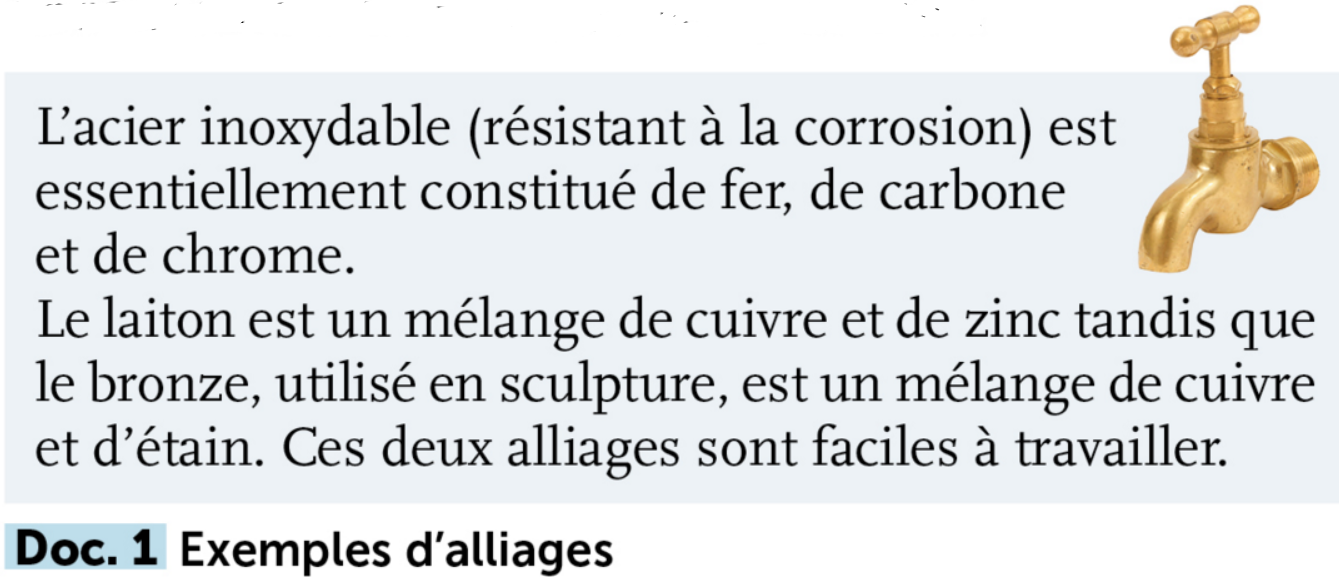
\includegraphics[scale=0.27]{img/qcm_doc1}	
%	\end{center}
%	
%	\begin{center}
%		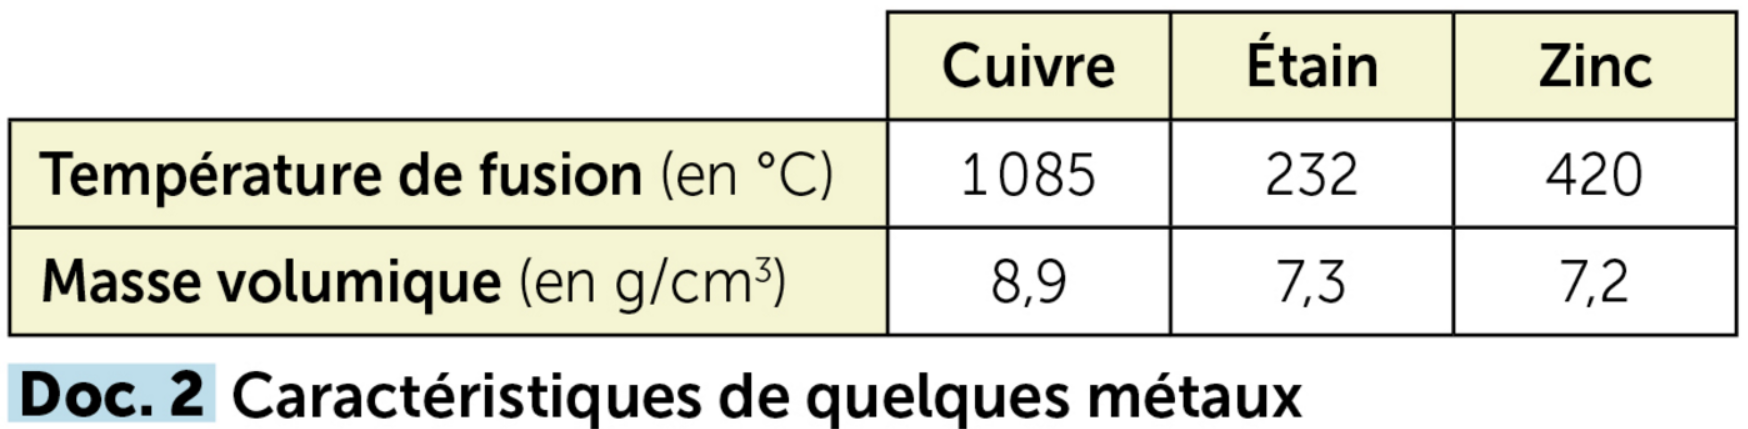
\includegraphics[scale=0.25]{img/qcm_doc2}	
%	\end{center}
%\end{multicols}
%
%
%	\begin{parts}
%		\part[] Ajouter du chrome à l'acier permet de le rendre plus :\\
%		\begin{oneparcheckboxes}
%			\choice oxydable
%			\choice dur	
%			\correctchoice résistant à la corrosion
%			
%		\end{oneparcheckboxes} 
%		
%		\part[] Ajouter du zinc au cuivre permet :\\
%		\begin{oneparcheckboxes}
%			\correctchoice d'abaisser la température de fusion.
%			\choice d'augmenter la masse volumique.
%			\choice de le rendre plus résistant.
%		\end{oneparcheckboxes}
%		
%		\part[] Un alliage de bronze composé de 20 \% d'étain et de 80 \% de cuivre a une masse volumique d'environ :\\
%		\begin{oneparcheckboxes}
%			\choice $\num{7.5} \ g/cm^3$
%			\choice $\num{8.1} \ g/cm^3$
%			\correctchoice $\num{8.6} \ g/cm^3$
%		\end{oneparcheckboxes}
%	
%	\end{parts}

\end{questions}